\documentclass[12pt, a4paper]{article}

\usepackage[utf8]{inputenc}
\usepackage[english, russian]{babel}
\usepackage{fancyhdr}
\usepackage{amsmath}
\usepackage{amsthm}
\usepackage{float}
\usepackage{graphicx}
\graphicspath{ {./} }
\usepackage{tabularx}
\newcolumntype{L}{>{\raggedright\arraybackslash}X}
\usepackage{pgfplots}
\usepackage{float}
\usepackage{xcolor}
\usepackage{hyperref}
\usepackage{multirow}
\pgfplotsset{width=\textwidth, compat=1.13}

\usepgfplotslibrary{external}
\usepgfplotslibrary{fillbetween}
\usepgfplotslibrary{statistics}
\usetikzlibrary{patterns.meta}


\graphicspath{{./}}
\newcommand{\Mod}[1]{\ \mathrm{mod}\ #1}

\usepackage[a4paper, margin=1.5cm]{geometry}

\usepackage{titlesec}
\titlelabel{\thetitle.\quad}

\pagestyle{plain}

\fancypagestyle{firstpage}{%
  \chead{
  МИНИСТЕРСТВО НАУКИ И ВЫСШЕГО ОБРАЗОВАНИЯ РОССИЙСКОЙ ФЕДЕРАЦИИ 
ФЕДЕРАЛЬНОЕ ГОСУДАРСТВЕННОЕ АВТОНОМНОЕ  
ОБРАЗОВАТЕЛЬНОЕ УЧРЕЖДЕНИЕ ВЫСШЕГО ОБРАЗОВАНИЯ\bigskip

«Национальный исследовательский университет ИТМО»\bigskip

ФИЗИЧЕСКИЙ ФАКУЛЬТЕТ 
}
\fancyfoot[CO]{Санкт-Петербург, 2023}%
}



\definecolor{aqua}{HTML}{003844}
\definecolor{peri}{HTML}{5EB1BF}
\definecolor{royal_blue}{HTML}{0A2463}
\definecolor{periwinkle}{HTML}{D8DCFF}
\definecolor{cerulean}{HTML}{247BA0}
\definecolor{bloodred}{HTML}{690500}
\definecolor{imperial_red}{HTML}{FB3640}
\definecolor{purple}{HTML}{511730}
\definecolor{tangerine}{HTML}{FFA781}

\definecolor{blue1}{HTML}{142459}
\definecolor{blue2}{HTML}{176BA0}
\definecolor{blue3}{HTML}{19AADE}
\definecolor{blue4}{HTML}{1AC936}
\definecolor{blue5}{HTML}{1DE4BD}
\definecolor{blue6}{HTML}{6DF0D2}

\definecolor{pink1}{HTML}{29066B}
\definecolor{pink2}{HTML}{7D3AC1}
\definecolor{pink3}{HTML}{AF4BCE}
\definecolor{pink4}{HTML}{DB4CB2}
\definecolor{pink5}{HTML}{EB548C}
\definecolor{pink6}{HTML}{EA7369}
\newtheorem*{task}{Условие}
\newtheorem*{finish}{Заключение}

%\tikzexternalize
\begin{document}
\newgeometry{top=1.6cm,bottom=1.6cm, left = 1.2cm, right = 1.2cm}

\topskip0pt
\vspace*{0.25\textheight}
\begin{center}
\textbf{\LARGE РАБОЧИЙ ПРОТОКОЛ И ОТЧЁТ }

\LARGE по лабораторной работе №1.04

\LARGE <<Исследование равноускоренного вращательного движения (маятник Обербека)>>

\end{center}
\vspace*{5cm}
\begin{flushright}
\begin{minipage}{.33\linewidth}
\textit{\textbf{Выполнил:}}\\
Хороших Дмитрий - P3217\\
\textit{\textbf{Преподаватель:}}\\
Коробков Максим Петрович
\end{minipage}
\end{flushright}


\thispagestyle{firstpage}
\newpage
\tableofcontents

\restoregeometry
\section{Введение}
\begin{enumerate}
\item Цель работы:

Проверить основной закон динамики вращения и теорему Гюйгенса-Штейнера (зависимость момента инерции от положения масс относительно оси вращения).

\item Задачи:
	\begin{enumerate}
		\item[1.]  Измерить время падения груза при разной массе груза и разном положении утяжелителей на крестовине.
		\item[2.] Рассчитать ускорение груза, угловое ускорение крестовины и мо-
мент силы натяжения нити.
		\item[3.] Рассчитать момент инерции крестовины с утяжелителями и момент силы трения
		\item[4.] Исследовать зависимость момента силы натяжения нити от углового ускорения, проверяя основной закон динамики вращения.
		\item[5.] Исследовать зависимость момента инерции от положения масс относительно оси вращения, проверяя теорему Штейнера-Гюйгенса.
	\end{enumerate}
		
\item Объект исследования:

Маятник Обербека

\item Схема установки:
\begin{figure}[h!]
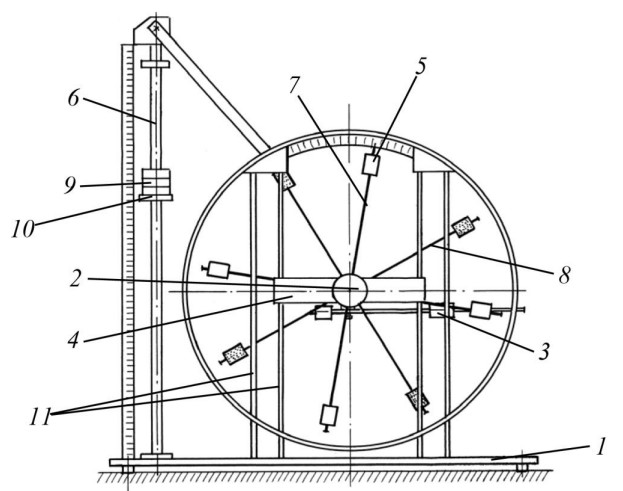
\includegraphics[width=0.5\textwidth]{pendulum.jpg}
\centering
\end{figure}

1. Основание
2. Рукоятка сцепления крестовин
3. Устройства принудительного трения
4. Поперечина
5. Груз крестовины
6. Трубчатая направляющая
7. Передняя крестовина
8. Задняя крестовина
9. Шайбы каретки
10. Каретка
11. Система передних стоек

\item Метод экспериментального исследования:

Многократный прямой замер времени падения каретки с шайбами.

\item Рабочие формулы:

Ускорени каретки с шайбами:
\begin{equation}
a = \frac{2*h}{t^2}
\end{equation}

Угловое ускорение крестовины:
\begin{equation}
\varepsilon = \frac{2*a}{d}
\end{equation}

Момент силы натяжения нити:
\begin{equation}
M = \frac{m*d}{2} * (g-a)
\end{equation}

Основной закон динамики вращения:
\begin{equation}
I\varepsilon = M - M_{\text{тр}}
\end{equation}

Зависиомсть инерции крестовины от расстояния между центрами грузов и осью вращения (в соответствии с теоремой Штейнера):
\begin{equation} \label{eq:1}
I = I_0 + 4m_{\text{ут}}R^2 
\end{equation}

\item Измерительные приборы:

\begin{center}

\begin{table}[h!]
\begin{tabular}{|l|l|l|l|l|}
\hline
№ п/п & Наименование & Тип & Используемый диапазон & Погрешность прибора\\
\hline
1 & Секундомер смартфона & Электронный & 0 - 999.99 сек  & 0.01 сек\\
\hline
\end{tabular}
\end{table}
\end{center}
\end{enumerate}
\section{Результаты измерений и их обработка}
\subsection{Прямые измерения}

Для каждого числа шайб (от 1 до 4) на каретке и для каждого положения грузов на крестовине (от 1 до 6 рисок) проведём 3 замера премени падения каретки с высоты $h=700$мм.

\begin{table}[h!]
\begin{center}
\begin{tabular}{|c|c|c|c|c|c|c|c|}
\hline
№ & Грузов на каретке & $t_{\text{1 риска}}$, с & $t_{\text{2 риска}}$, с & $t_{\text{3 риска}}$, с & $t_{\text{4 риска}}$, с & $t_{\text{5 риска}}$, с & $t_{\text{6 риска}}$, с\\
\hline
1 & $1*m $ &4.99 & 6.10 & 6.10 & 6.99 & 9.12 & 10.20\\ 
\hline 
2 & $1*m $ &4.96 & 5.56 & 6.36 & 7.10 & 8.93 & 10.15\\ 
\hline 
3 & $1*m $ &4.93 & 6.06 & 6.16 & 7.05 & 9.15 & 8.83\\ 
\hline 
4 & $2*m $ &3.70 & 4.18 & 5.03 & 5.72 & 5.93 & 7.18\\ 
\hline 
5 & $2*m $ &3.55 & 4.40 & 4.96 & 5.19 & 6.40 & 6.66\\ 
\hline 
6 & $2*m $ &3.72 & 4.53 & 5.03 & 5.83 & 5.92 & 7.23\\ 
\hline 
7 & $3*m $ &3.10 & 3.63 & 3.95 & 4.68 & 5.16 & 5.69\\ 
\hline 
8 & $3*m $ &3.20 & 3.35 & 4.06 & 4.42 & 5.00 & 5.82\\ 
\hline 
9 & $3*m $ &3.07 & 3.59 & 3.88 & 4.58 & 5.33 & 5.63\\ 
\hline 
10 & $4*m $ &2.40 & 3.06 & 3.56 & 4.03 & 4.40 & 5.00\\ 
\hline 
11 & $4*m $ &2.68 & 3.05 & 3.40 & 3.99 & 4.51 & 4.90\\ 
\hline 
12 & $4*m $ &2.62 & 3.03 & 3.42 & 3.88 & 4.37 & 5.10\\ 
\hline 
\end{tabular}
\caption{Результаты прямых измерений времени падения}
\end{center}
\label{tab:1}
\end{table}
\newpage
\subsection{Обработка прямых измерений}
Найдём среднее время падения каретки для всех масс шайб и всех положений утяжелителей на крестовине. Также рассчитаем абсолютную погрешность среднего значения времени $\Delta t$.
\begin{table}[!h]
\begin{center}
\begin{tabular}{|c|c|c|c|c|c|c|c|}
\hline
Грузов на каретке & & 1 риска & 2 риски & 3 риски & 4 риски & 5 рисок & 6 рисок \\
\hline
\multirow{2}{*}{$1 m $} & $t_{\text{ср}}$, c &4.96 & 5.91 & 6.21 & 7.05 & 9.07 & 9.73\\ 
&$\Delta t$, c &0.07 & 0.75 & 0.34 & 0.14 & 0.30 & 1.93\\ 
\hline 
\multirow{2}{*}{$2 m $} & $t_{\text{ср}}$, c &3.66 & 4.37 & 5.01 & 5.58 & 6.08 & 7.02\\ 
&$\Delta t$, c &0.23 & 0.44 & 0.10 & 0.85 & 0.68 & 0.78\\ 
\hline 
\multirow{2}{*}{$3 m $} & $t_{\text{ср}}$, c &3.12 & 3.52 & 3.96 & 4.56 & 5.16 & 5.71\\ 
&$\Delta t$, c &0.17 & 0.38 & 0.23 & 0.33 & 0.41 & 0.24\\ 
\hline 
\multirow{2}{*}{$4 m $} & $t_{\text{ср}}$, c &2.57 & 3.05 & 3.46 & 3.97 & 4.43 & 5.00\\ 
&$\Delta t$, c &0.37 & 0.04 & 0.22 & 0.19 & 0.18 & 0.25\\ 
\hline 

\end{tabular}
\caption{Среднее время падения каретки и его абсолютная погрешность}
\end{center}
\label{tab:2}
\end{table}

\subsection{Косвенные измерения}
Используя найденные значения $t_\text{ср}$ рассчитаем ускорение $a$ груза, угловое ускорение $\varepsilon$ крестовины, момент $M$ силы натяжения
нити а также их абсолютную погрешность.

\begin{table}[h!]
\begin{center}
\begin{tabular}{|c|c|c|c|c|c|c|c|}
\hline
Грузов на каретке & & 1 риска & 2 риски & 3 риски & 4 риски & 5 рисок & 6 рисок \\
\hline
\multirow{6}{*}{$1 m $} & $a$, мм/$c^2$ &56.91 & 40.13 & 36.34 & 28.19 & 17.03 & 14.80\\[5pt] 
\cline{2-8} 
&$\Delta a$, мм/$c^2$&1.72 & 10.15 & 3.96 & 1.10 & 1.11 & 5.87\\[5pt] 
\cline{2-8} 
& $\varepsilon$, рад/$c^2$ &2.47 & 1.74 & 1.58 & 1.23 & 0.74 & 0.64\\[5pt] 
\cline{2-8} 
&$\Delta \varepsilon$, рад/$c^2$ &0.08 & 0.44 & 0.17 & 0.05 & 0.05 & 0.26\\[5pt] 
\cline{2-8} 
&$M$, Н*мм &59.87 & 59.97 & 60.00 & 60.05 & 60.11 & 60.13\\[5pt] 
\cline{2-8} 
&$\Delta M$, Н*мм &0.69 & 0.69 & 0.69 & 0.69 & 0.69 & 0.69\\[5pt] 
\cline{2-8} 
\hline 
\multirow{6}{*}{$2 m $} & $a$, мм/$c^2$ &104.70 & 73.31 & 55.85 & 44.96 & 37.83 & 28.38\\[5pt] 
\cline{2-8} 
&$\Delta a$, мм/$c^2$&13.22 & 14.74 & 2.24 & 13.69 & 8.47 & 6.33\\[5pt] 
\cline{2-8} 
& $\varepsilon$, рад/$c^2$ &4.55 & 3.19 & 2.43 & 1.95 & 1.64 & 1.23\\[5pt] 
\cline{2-8} 
&$\Delta \varepsilon$, рад/$c^2$ &0.58 & 0.64 & 0.10 & 0.60 & 0.37 & 0.28\\[5pt] 
\cline{2-8} 
&$M$, Н*мм &108.66 & 109.02 & 109.21 & 109.33 & 109.41 & 109.52\\[5pt] 
\cline{2-8} 
&$\Delta M$, Н*мм &1.24 & 1.24 & 1.23 & 1.24 & 1.24 & 1.24\\[5pt] 
\cline{2-8} 
\hline 
\multirow{6}{*}{$3 m $} & $a$, мм/$c^2$ &143.51 & 112.78 & 89.13 & 67.33 & 52.51 & 42.89\\[5pt] 
\cline{2-8} 
&$\Delta a$, мм/$c^2$&15.54 & 24.07 & 10.14 & 9.62 & 8.33 & 3.62\\[5pt] 
\cline{2-8} 
& $\varepsilon$, рад/$c^2$ &6.24 & 4.90 & 3.88 & 2.93 & 2.28 & 1.86\\[5pt] 
\cline{2-8} 
&$\Delta \varepsilon$, рад/$c^2$ &0.68 & 1.05 & 0.44 & 0.42 & 0.36 & 0.16\\[5pt] 
\cline{2-8} 
&$M$, Н*мм &157.12 & 157.62 & 158.01 & 158.36 & 158.60 & 158.76\\[5pt] 
\cline{2-8} 
&$\Delta M$, Н*мм &1.78 & 1.81 & 1.78 & 1.79 & 1.79 & 1.78\\[5pt] 
\cline{2-8} 
\hline 
\multirow{6}{*}{$4 m $} & $a$, мм/$c^2$ &212.51 & 150.83 & 116.94 & 88.98 & 71.45 & 56.00\\[5pt] 
\cline{2-8} 
&$\Delta a$, мм/$c^2$&60.62 & 3.81 & 14.64 & 8.66 & 5.91 & 5.56\\[5pt] 
\cline{2-8} 
& $\varepsilon$, рад/$c^2$ &9.24 & 6.56 & 5.08 & 3.87 & 3.11 & 2.43\\[5pt] 
\cline{2-8} 
&$\Delta \varepsilon$, рад/$c^2$ &2.64 & 0.18 & 0.64 & 0.38 & 0.26 & 0.24\\[5pt] 
\cline{2-8} 
&$M$, Н*мм &204.54 & 205.86 & 206.58 & 207.18 & 207.55 & 207.88\\[5pt] 
\cline{2-8} 
&$\Delta M$, Н*мм &2.63 & 2.31 & 2.33 & 2.33 & 2.33 & 2.33\\[5pt] 
\cline{2-8} 
\hline 


\end{tabular}
\caption{Характеристики движения груза и крестовины}
\end{center}
\label{tab:3}
\end{table}


\clearpage
\subsection{Обработка косвенных измерений}
Для каждого положения утяжелителей на крестовине в координатах $M$ - $\varepsilon$ нанесём точки зависимостей $M(\varepsilon)$.

С помощью метода наименьших квадратов (МНК) рассчитаем момент инерции $I$ и момент силы трения $M_{\text{тр}}$ а также их абсолютную погрешность. Перенесём полученные значения в таблицу \ref{tab:5} и построим прямые $M = M_{\text{тр}} + I\varepsilon$ на рисунке \ref{gr:1}.
\begin{figure}[H]
\begin{tikzpicture}
\begin{axis}[
	axis lines = left,
	xlabel = \(\varepsilon \text{, рад/}c^2\),
	ylabel = {\(M \text{, Н*мм}\)},
	ymin=40,	
	xmin=0,
	xmax=12,
	grid=both,
    grid style={line width=.1pt, draw=gray!10},
    major grid style={line width=.2pt,draw=gray!50},
    minor tick num=5,
	axis x line = bottom,
	axis line style ={line width = .3pt},
	ymax=220,
	legend style={at={(0.8, 0.3)},anchor=west}
	]


\addplot[only marks,pink1, mark size =2pt, error bars/.cd, y dir=both, y explicit, x dir=both, x explicit, error mark options={
      pink1,
      mark size=0.4pt,
      line width=4pt
    }, error bar style={fill=pink1,scale=2, line width=1pt}] table [y = y, y error = y-err, x = x, x error = x-err,  col sep=comma] {momentum-accel1.csv};


\addplot[pink1, domain=0:10] { 21.61131914653501*x+10.953548551998958};


\addplot[only marks,pink2, mark size =2pt, error bars/.cd, y dir=both, y explicit, x dir=both, x explicit, error mark options={
      pink2,
      mark size=0.4pt,
      line width=4pt
    }, error bar style={fill=pink2,scale=2, line width=1pt}] table [y = y, y error = y-err, x = x, x error = x-err,  col sep=comma] {momentum-accel2.csv};


\addplot[pink2, domain=0:10] { 30.057864246822078*x+9.931389597103522};


\addplot[only marks,pink3, mark size =2pt, error bars/.cd, y dir=both, y explicit, x dir=both, x explicit, error mark options={
      pink3,
      mark size=0.4pt,
      line width=4pt
    }, error bar style={fill=pink3,scale=2, line width=1pt}] table [y = y, y error = y-err, x = x, x error = x-err,  col sep=comma] {momentum-accel3.csv};


\addplot[pink3, domain=0:10] { 40.457300178469794*x+2.286167693169117};


\addplot[only marks,pink4, mark size =2pt, error bars/.cd, y dir=both, y explicit, x dir=both, x explicit, error mark options={
      pink4,
      mark size=0.4pt,
      line width=4pt
    }, error bar style={fill=pink4,scale=2, line width=1pt}] table [y = y, y error = y-err, x = x, x error = x-err,  col sep=comma] {momentum-accel4.csv};


\addplot[pink4, domain=0:10] { 54.88550594668295*x+-3.16431183711496};


\addplot[only marks,pink5, mark size =2pt, error bars/.cd, y dir=both, y explicit, x dir=both, x explicit, error mark options={
      pink5,
      mark size=0.4pt,
      line width=4pt
    }, error bar style={fill=pink5,scale=2, line width=1pt}] table [y = y, y error = y-err, x = x, x error = x-err,  col sep=comma] {momentum-accel5.csv};


\addplot[pink5, domain=0:10] { 63.2859845328355*x+10.911128508714885};


\addplot[only marks,pink6, mark size =2pt, error bars/.cd, y dir=both, y explicit, x dir=both, x explicit, error mark options={
      pink6,
      mark size=0.4pt,
      line width=4pt
    }, error bar style={fill=pink6,scale=2, line width=1pt}] table [y = y, y error = y-err, x = x, x error = x-err,  col sep=comma] {momentum-accel6.csv};


\addplot[pink6, domain=0:10] { 81.98760575498524*x+7.463481783116788};


\legend{1 Риска,$M_{\text{1}}(\varepsilon)$, 2 Риски,$M_{\text{2}}(\varepsilon)$, 3 Риски,$M_{\text{3}}(\varepsilon)$, 4 Риски,$M_{\text{4}}(\varepsilon)$, 5 Рисок,$M_{\text{5}}(\varepsilon)$,6 Рисок, $M_{\text{6}}(\varepsilon)$}

\end{axis}
\end{tikzpicture}
\caption{Графики зависимости $M$ от $\varepsilon$ для различных положений утяжелителей на крестовине.}
\label{gr:1}
\end{figure}


\begin{table}[!h]
\begin{center}
\begin{tabular}{|c|c|c|c|c|}
\hline
Число рисок& $I$ & $\Delta I$ & $M_{\text{тр}}$ & $\Delta M_{\text{тр}}$\\
\hline
1 & 21.61 & 3.90 & 10.95 & 23.97\\ 
\hline 
2 & 30.06 & 1.66 & 9.93 & 7.43\\ 
\hline 
3 & 40.46 & 5.70 & 2.29 & 19.99\\ 
\hline 
4 & 54.89 & 4.93 & -3.16 & 13.24\\ 
\hline 
5 & 63.29 & 5.59 & 10.91 & 11.90\\ 
\hline 
6 & 81.99 & 2.09 & 7.46 & 3.53\\ 
\hline 


\end{tabular}
\caption{Момент инерции и момент силы трения, полученные по МНК.}
\end{center}
\label{tab:4}
\end{table}

\begin{table}[!h]
\begin{center}
\begin{tabular}{|c|c|c|c|c|c|c|}
\hline
& 1 риска & 2 риски & 3 риски & 4 риски & 5 рисок & 6 рисок \\
\hline
$I$, г*$\text{м}^2$ &21.61 & 30.06 & 40.46 & 54.89 & 63.29 & 81.99\\ 
\hline 
 $R$, $\text{мм}$ &77 & 102 & 127 & 152 & 177 & 202\\ 
\hline 
$R^2$, $\text{мм}^2$ &5929 & 10404 & 16129 & 23104 & 31329 & 40804\\ 
\hline 


\end{tabular}
\caption{Момент инерции и расстояние от центра крестовины до утяжелителей.}
\end{center}
\label{tab:6}
\end{table}

Рассчитаем расстояния $R$ от центра крестовины до утяжелителей и внесём  в таблицу \ref{tab:6} значения $I$, $R$, $R^2$.

На основании полученных значений в координатах $I$ - $R^2$ на рисунке \ref{gr:2} отметим экспери-
ментальные точки зависимости $I(R^2)$.
\begin{figure}[H]
\begin{tikzpicture}
\begin{axis}[
	axis lines = left,
	ylabel = \(I \text{, г}*\text{м}^2\),
	xlabel = {\(R^2,10^{3}*\text{мм}^2\)},
	ymin=0,	
	xmin=0,
	xmax=45,
	grid=both,
    grid style={line width=.1pt, draw=gray!10},
    major grid style={line width=.2pt,draw=gray!50},
    minor tick num=5,
	axis x line = bottom,
	axis line style ={line width = .3pt},
	ymax=90,
	legend style={at={(0.8, 0.3)},anchor=west}
	]




\addplot[only marks,blue1, mark size =2pt, error bars/.cd, y dir=both, y explicit, x dir=both, x explicit, error mark options={
      blue1,
      mark size=0.4pt,
      line width=4pt
    }, error bar style={fill=blue1,scale=2, line width=1pt}] table [y = y, y error = y-err, x = x,  col sep=comma] {inertia-radius1.csv};


\addplot[only marks,blue2, mark size =2pt, error bars/.cd, y dir=both, y explicit, x dir=both, x explicit, error mark options={
      blue2,
      mark size=0.4pt,
      line width=4pt
    }, error bar style={fill=blue2,scale=2, line width=1pt}] table [y = y, y error = y-err, x = x,  col sep=comma] {inertia-radius2.csv};


\addplot[only marks,blue3, mark size =2pt, error bars/.cd, y dir=both, y explicit, x dir=both, x explicit, error mark options={
      blue3,
      mark size=0.4pt,
      line width=4pt
    }, error bar style={fill=blue3,scale=2, line width=1pt}] table [y = y, y error = y-err, x = x,  col sep=comma] {inertia-radius3.csv};


\addplot[only marks,blue4, mark size =2pt, error bars/.cd, y dir=both, y explicit, x dir=both, x explicit, error mark options={
      blue4,
      mark size=0.4pt,
      line width=4pt
    }, error bar style={fill=blue4,scale=2, line width=1pt}] table [y = y, y error = y-err, x = x,  col sep=comma] {inertia-radius4.csv};


\addplot[only marks,blue5, mark size =2pt, error bars/.cd, y dir=both, y explicit, x dir=both, x explicit, error mark options={
      blue5,
      mark size=0.4pt,
      line width=4pt
    }, error bar style={fill=blue5,scale=2, line width=1pt}] table [y = y, y error = y-err, x = x,  col sep=comma] {inertia-radius5.csv};


\addplot[only marks,blue6, mark size =2pt, error bars/.cd, y dir=both, y explicit, x dir=both, x explicit, error mark options={
      blue6,
      mark size=0.4pt,
      line width=4pt
    }, error bar style={fill=blue6,scale=2, line width=1pt}] table [y = y, y error = y-err, x = x,  col sep=comma] {inertia-radius6.csv};


\addplot[peri, domain=0:45] {1.696148200241765*x+12.614858463942907};


\legend{1 Риска, 2 Риски, 3 Риски, 4 Риски, 5 Рисок,6 Рисок, $I(R^2)$}

\end{axis}
\end{tikzpicture}
\caption{График зависимости $I$ от $R^2$.}
\label{gr:2}
\end{figure}

При помощи МНК из формулы \eqref{eq:1} определяем значения $I_0$, $m_{\text{ут}}$ и c учётом погрешности:
\begin{equation*}
\begin{aligned}
 I_0 &= 12.61 \pm 3.4 \text{ г}*\text{м}^2 \\
 m_{\text{ут}} &= 424.04 \pm 35.05 \text{ г} \\
  \end{aligned}
\end{equation*}

Заметим, что реальное значение $ m_{\text{ут}}$ равно:
\begin{equation*}
 m_{\text{ут}} = 408 \pm 0.5 \text{ г}
\end{equation*}

\section{Вывод}
Таким образом, в ходе выполнения лабораторной работы удалось, измерив время падения каретки, соединённой с маятником Обербека, при различных грузах и положениях утяжелителях, подтвердить:
\begin{itemize}
\item[1.] Линейную зависимость момента силы натяжения от углового ускорения (Основной закон динамики вращения). 

На рисунке \ref{gr:1} легко видеть, что, несмотря на высокую погрешность, зависимость $M(\varepsilon)$ линейна, что сходится с теоретическими выводами.

\item[2.] Квадратичную зависимость момента инерции от расстояния между массами и осью вращения (Теорема Гюйгенса-Штейнера). 

На рисунке \ref{gr:2} график, построенный в осях $I$-$R^2$ , представляет из себя прямую. Следовательно, зависимость $I(R)$ - квадратична.

Правильность заключения подтверждается, помимо теоретических выводов, и фактом получения близкого к реальному значению массы утяжелителя $m_{\text{ут}}$.


\end{itemize}


\section{Приложение}
Проект этой лабораторной работы, содержащий файлы с Python-кодом, использованным для вычислений и исходные TeX-файлы доступен по ссылке: \url{https://github.com/Dimankarp/Studies/tree/main/Physics/Lab2}.

\end{document}



